\documentclass[12pt,a4paper]{article}

% Кодування/мови — в такому порядку
\usepackage[utf8]{inputenc}
\usepackage[T2A]{fontenc}
\usepackage[ukrainian]{babel}
\usepackage{cmap}            % коректний копіпаст з PDF (текстовий шар)
% (бажано мати шрифти cm-super у дистрибутиві)

\usepackage{geometry}
\geometry{left=2cm,right=2cm,top=2cm,bottom=2cm}

\usepackage{graphicx}
\usepackage{array,multirow,booktabs,makecell}
\usepackage{caption}
\renewcommand{\thetable}{\arabic{table}}
\usepackage[table]{xcolor} % <-- це дає \rowcolor і \cellcolor
\captionsetup[table]{name=Таблиця}

\usepackage{amsmath}
\usepackage{pdflscape}
\usepackage{xcolor}

% Гіперпосилання — тримай наприкінці пакетів, з unicode
\usepackage[unicode]{hyperref}

\renewcommand\cellalign{tc}
\renewcommand\theadalign{cc}
\renewcommand{\arraystretch}{1.25}

\begin{document}

    \begin{titlepage}

        % Картинка шапки (по центру, з відступом від верху)
        \begin{center}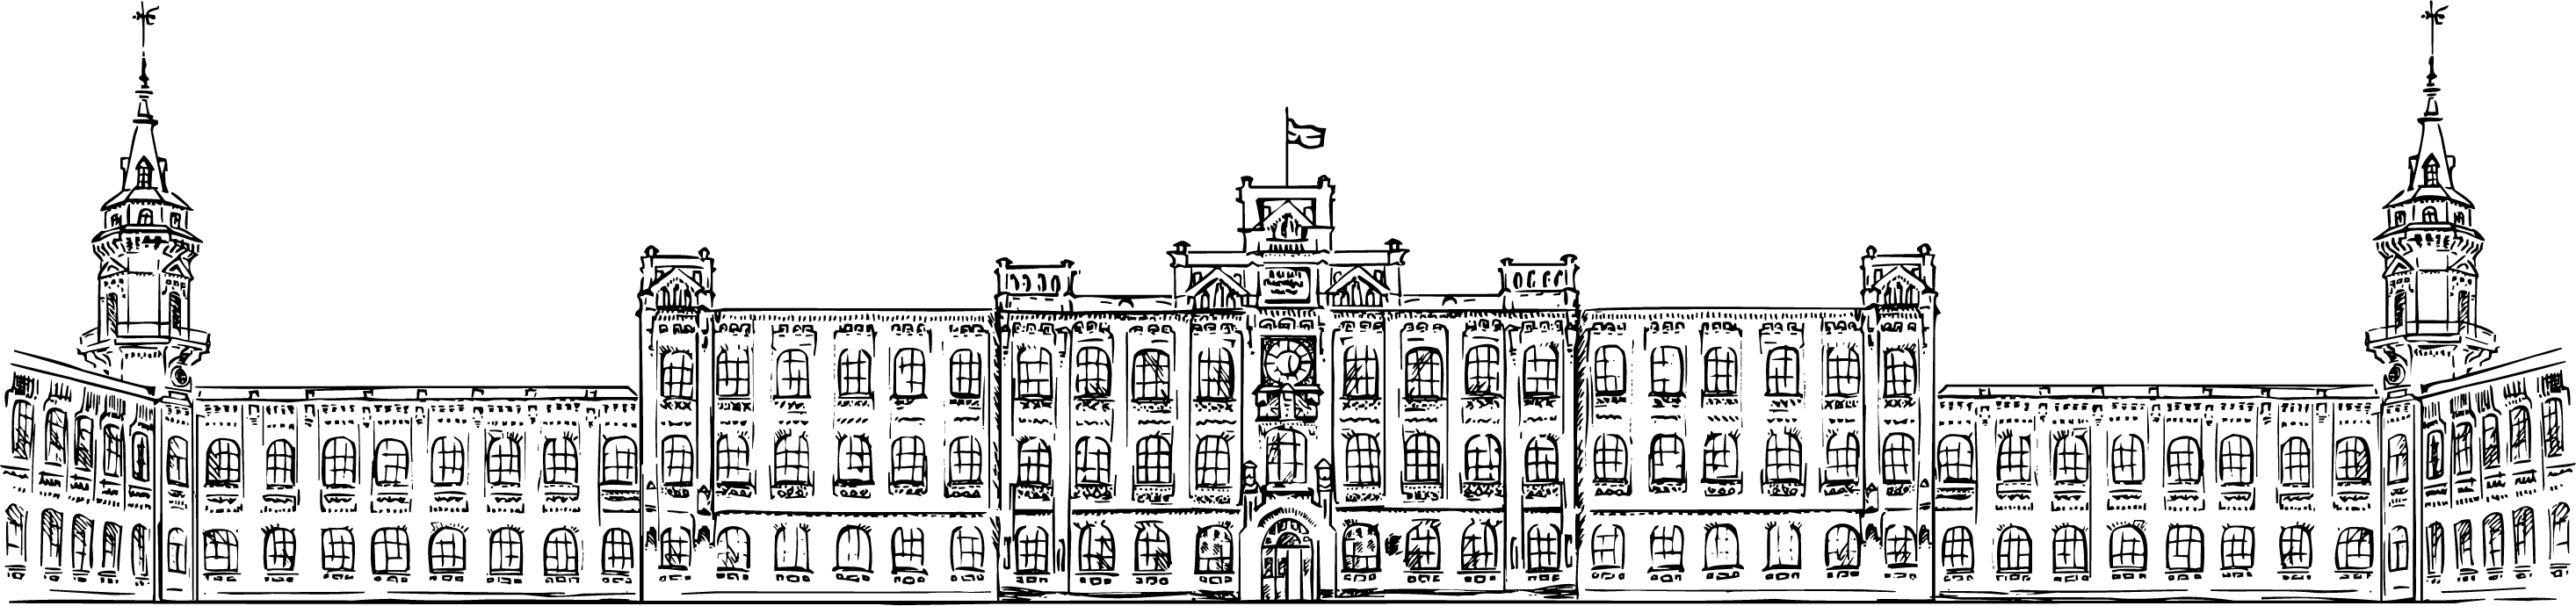
\includegraphics[width=0.7\textwidth]{../../../TITLES/letterhead.png}\end{center}

        \begin{center}
            \large Національний технічний університет України\\
            «Київський політехнічний інститут імені Ігоря Сікорського»\\[1em]
            Факультет інформатики та обчислювальної техніки\\
            Кафедра обчислювальної техніки
        \end{center}

        \vfill

        \begin{center}
            \textbf{\LARGE Теорія електричних кіл та сигналів}\\[2em]
            \textbf{\Large Лабораторна робота №4}\\
            «Дослідження однофазного електричного кола змінного струму»
        \end{center}

        \vfill

        \begin{flushright}
            Виконав: студент 2 курсу ФІОТ, гр. ІО-41\\
            \textit{Давидчук А.~М.}\\[1em]
            Перевірив: \textit{Лободзинський В.~Ю.}
        \end{flushright}

        \vfill

        \begin{center}Київ --- 2025\end{center}

    \end{titlepage}

    \setlength{\parindent}{0pt}

    \textbf{\underline{Тема:}} «Дослідження однофазного електричного кола змінного струму».

    \vspace{1em}

    \textbf{\underline{Мета:}} Дослідити характеристики однофазного електричного кола змінного
    струму та навчитися визначати параметри його елементів (активних,
    індуктивних, ємнісних) за допомогою вимірювальних приладів (вольтметра,
    амперметра, ватметра).
    Навчитися використовувати вимірювальні прилади для вимірювання
    напруги, струму, потужності, кута зсуву фаз.
    Навчитись визначати активні, реактивні та повні опори, кути зсуву фаз.
    Навчитись будувати суміщені векторні діаграми струмів та напруг
    електричних кіл синусоїдного струму.

    \begin{center} \textbf{\Large Практична частина} \end{center}

    \setlength{\parindent}{1.5em}

    Усі розрахунки було проведено за допомогою мови програмування Python (вихідний код додано разом із звітом).

    \begin{center} \textbf{\large Завдання №1 (офлайн вимірювання)} \end{center}

    Під час проведення офлайн заняття, ми скали таку електричну схему:



    %Моя група: ІО-41, мій порядковий номер у групі: 6. Звідси $N = 6$, $S = 1$.
    %Звідси загальна структурна схема електричного кола:

    \begin{figure}[h!]

        \renewcommand{\thefigure}{\arabic{figure}} % робимо "3.1", "3.2" і т.д.

        \centering
        % Підставляєте потрібний шлях та розмір зображення:
        
\includegraphics[width=0.3\textwidth]{scheme0.png}
        % Підпис (зазвичай під малюнком):
        \caption{Структурна схема електричного кола з послідовним сполученням елементів}
        % Мітка для посилань у тексті (\ref{fig:...})
        \label{fig1:scheme0}

    \end{figure}

    Та проводили виміри сили струму, напруг, потужностей та зсуву фаз. Результат вимірів винесено в таблицю:

    \begin{center}
    \setlength{\tabcolsep}{8pt}
    \begin{tabular}{|
    p{2.3cm}|
    p{0.5cm}|p{0.8cm}|
    p{0.5cm}|p{1.1cm}|
    p{0.5cm}|p{0.8cm}|
    p{1.1cm}|p{1.1cm}|p{1.1cm}|p{1.4cm}|}
    \hline
    \multicolumn{7}{|c|}{\textbf{Дані вимірювання}} &
    \multicolumn{4}{c|}{\textbf{Результати обчислень}} \\
    \cline{8-11}
    \multicolumn{7}{|c|}{} &
    \textbf{Z} & \textbf{R} & \textbf{X} & $\underline{Z}=Z e^{j\varphi}$ \\
    \hline
    \makecell[c]{Резистор} &
    \makecell{$U_R$\\В} & 2,95 &
    $\varphi_R$ & 0 &
    \makecell{$P_R$\\Вт} & 0,13 &
    73,75 & & & \\
    \hline
    \makecell[c]{Індуктивна\\котушка} &
    \makecell{$U_L$\\В} & 5,60 &
    $\varphi_L$ & 51 &
    \makecell{$P_L$\\Вт} & 0,14 &
    140 & & & \\
    \hline
    \makecell[c]{Конденсатор} &
    \makecell{$U_C$\\В} & 13,12 &
    $\varphi_C$ & -86 &
    \makecell{$P_C$\\Вт} & 0,03 &
    328 & & & \\
    \hline
    \makecell[c]{Все коло} &
    \makecell{$U$\\В} & 10,40 &
    $\varphi$ & 49 &
    \makecell{$P$\\Вт} & 0,27 &
    260 & & & \\
    \cline{2-11}
    \multicolumn{1}{|c|}{} &
    \makecell{$I$\\А} &
    \multicolumn{5}{c|}{} &   % <-- колонки 3–7 (закінчується вертикальною лінією)
    \multicolumn{4}{c|}{} \\  % <-- колонки 8–11
    \hline
    \end{tabular}
    \end{center}

    \newpage

    \begin{center} \textbf{\large Завдання №2 (адання на навчально-дослідну роботу студента)} \end{center}

    В цьому завданні, необхідно побудувати схему зі джерелом змінної напруги $u(t) = U_m \sin(\omega t + \alpha^{\circ})$, з частотою $f$ Гц, до якого приєднаний двополюсник з Навантаженням $Z_H$:

    \begin{figure}[h!]

        \renewcommand{\thefigure}{\arabic{figure}} % робимо "3.1", "3.2" і т.д.

        \centering
        % Підставляєте потрібний шлях та розмір зображення:
        
\includegraphics[width=0.3\textwidth]{graph2.png}
        % Підпис (зазвичай під малюнком):
        \caption{Структурна схема електричного кола}
        % Мітка для посилань у тексті (\ref{fig:...})

    \end{figure}

    Обчислимо параметри схеми за допомогою формул:

    \[
    U_m = 10 + S,\ \text{В}
    \]
    \[
    \alpha = 90 - 2 \cdot N,\ \text{град};
    \]
    \[
    f = S \cdot 100 + N,\ \text{Гц};
    \]
    \[
    Z_H = (N + 5 + 10 \cdot S) + j(2 \cdot N + 10 \cdot S)\cdot k,\ \text{Ом}.
    \]

    Обчислення як і для попереднього завдання проводились за допомгою мови програмування Python (файл \texttt{task2.py} буде доданий разом із звітом).

    А також будемо вимірювати покази приладів (амперметра, вольтметра, осцилографа та ваттметра), обчислимо зсув фаз та всі розрахункові дані занесемо до таблиці:

    \begin{center}
    \begin{tabular}{|
    >{\centering\arraybackslash}p{3.2cm}|
    >{\centering\arraybackslash}p{3.2cm}|
    >{\centering\arraybackslash}p{3.2cm}|
    >{\centering\arraybackslash}p{3.2cm}|}
    \hline
    \rowcolor[HTML]{D9D9D9}\multicolumn{4}{|c|}{\textbf{Параметри джерела живлення}}\\
    \hline
    $U_m$, \text{В} & $U$, \text{В} & $\alpha$, \text{град} & $f$, \text{Гц} \\
    \hline
    11 & 7,778 & 78 & 106 \\
    \hline
    \rowcolor[HTML]{D9D9D9}\multicolumn{4}{|c|}{\textbf{Навантаження}}\\
    \hline
    \multicolumn{1}{|l|}{$Z_H = 21 + 22j$} & \multicolumn{3}{l|}{} \\
    \hline
    $R$, \text{Ом} & $L$, \text{Гн} & $C$, \text{Ф} &  \\
    \hline
    21 & 0,033 & - &  \\
    \hline
    \rowcolor[HTML]{D9D9D9}\multicolumn{4}{|c|}{\textbf{Покази приладів}}\\
    \hline
    $I$, \text{А} & $U$, \text{В} & $P$, \text{Вт} & $\varphi$, \text{град} \\
    \hline
    0,255 & 7,76 & 1,364 & 46,25 \\
    \hline
    \end{tabular}
    \end{center}

    \newpage

    Ось фото побудованої схеми разом із показами приладів:

    \begin{figure}[h!]

        \renewcommand{\thefigure}{\arabic{figure}} % робимо "3.1", "3.2" і т.д.

        \centering
        % Підставляєте потрібний шлях та розмір зображення:
        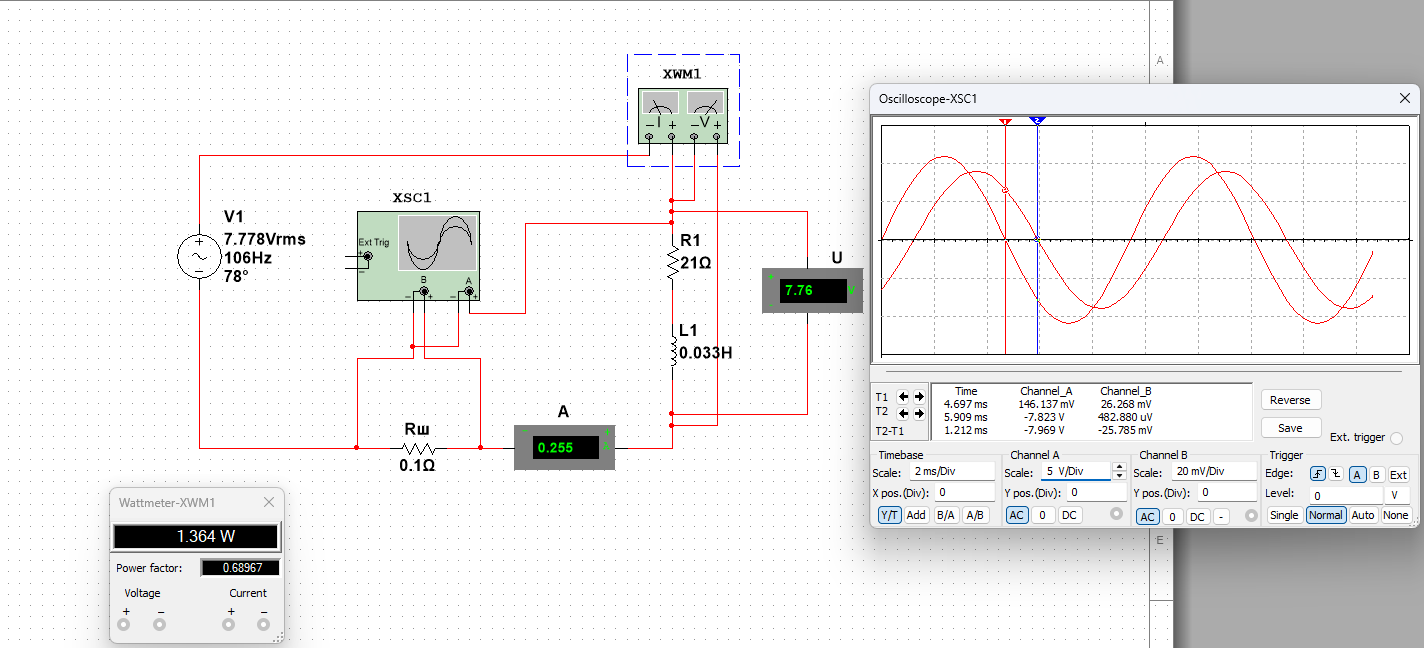
\includegraphics[width=1.0\textwidth]{mulitism_scheme.png}
        % Підпис (зазвичай під малюнком):
        \caption{Електричне коло та значення приладів у програмі Multisim}
        % Мітка для посилань у тексті (\ref{fig:...})

    \end{figure}

    У таблиці як видно, зсув фаз між напругою та струмом буде додатньої, через наявність котукшки індуктивності: сила струму відстає від напруги.

    Безпосередньо, зсув фаз порахував за формулою:

    \[
    \varphi = \frac{360 \cdot \Delta T}{T}
    \]

    де

    \[
    T = \frac{1}{f}
    \]
    а, $\Delta T$ брав із графіків осцилографа.



    %\textbf{Висновок:} 

\end{document}